% User manual for a fictional espresso machine (Morvale ES-300). English, A5-like feel on A4, 3 pages.
% Features: tikz parts drawing with numbered callouts and NO caption (on purpose), WARNING/CAUTION boxes,
% numbered descaling procedure, troubleshooting table, technical specification table.
\documentclass[10pt,a4paper]{article}
\usepackage[T1]{fontenc}
\usepackage[utf8]{inputenc}
\usepackage[scaled=0.92]{helvet}
\renewcommand{\familydefault}{\sfdefault}
\usepackage[english]{babel}
\usepackage[margin=2.1cm,top=2.3cm,bottom=2.2cm]{geometry}
\usepackage{xcolor}
\usepackage{tikz}
\usetikzlibrary{calc}
\usepackage{tcolorbox}
\tcbuselibrary{skins}
\usepackage{enumitem}
\usepackage{booktabs}
\usepackage{array}
\usepackage{tabularx}
\usepackage{titlesec}
\usepackage{fancyhdr}
\usepackage{lastpage}
\usepackage{needspace}
\usepackage{siunitx}
\usepackage{caption}
\captionsetup{font=small, labelfont=bf, labelsep=colon, justification=raggedright, singlelinecheck=false}
\sisetup{mode=text}

\definecolor{brand}{HTML}{7A3E1D}
\definecolor{warnred}{HTML}{B3261E}
\definecolor{cautionamber}{HTML}{C77700}

\setlength{\parindent}{0pt}
\setlength{\parskip}{0.45em}
\titleformat{\section}{\Large\bfseries\color{brand}}{\thesection}{0.7em}{}[{\color{brand}\titlerule}]
\titleformat{\subsection}{\large\bfseries}{\thesubsection}{0.6em}{}
\titlespacing*{\section}{0pt}{1.4em}{0.6em}
\titlespacing*{\subsection}{0pt}{1em}{0.3em}

\pagestyle{fancy}
\fancyhf{}
\renewcommand{\headrulewidth}{0.4pt}
\fancyhead[L]{\small\textbf{Morvale ES-300} \textperiodcentered{} User manual}
\fancyhead[R]{\small Version 1.4 \textperiodcentered{} 09/2026}
\fancyfoot[L]{\small Morvale Home Appliances Ltd., Fictional Street 1, Exampleville}
\fancyfoot[R]{\small Page \thepage{} of \pageref{LastPage}}

% Safety boxes -------------------------------------------------------------------------
\newtcolorbox{warnbox}{enhanced, colback=warnred!6, colframe=warnred, boxrule=0.6pt, left=8pt, right=8pt,
  top=4pt, bottom=4pt, fonttitle=\bfseries, title={\textbf{WARNING}}, coltitle=white, colbacktitle=warnred,
  attach boxed title to top left={yshift=-2mm, xshift=3mm}, boxed title style={sharp corners, boxrule=0pt, size=small}}
\newtcolorbox{cautionbox}{enhanced, colback=cautionamber!7, colframe=cautionamber, boxrule=0.6pt, left=8pt,
  right=8pt, top=4pt, bottom=4pt, fonttitle=\bfseries, title={\textbf{CAUTION}}, coltitle=white,
  colbacktitle=cautionamber, attach boxed title to top left={yshift=-2mm, xshift=3mm},
  boxed title style={sharp corners, boxrule=0pt, size=small}}
\newtcolorbox{notebox}{colback=black!4, colframe=black!40, boxrule=0.4pt, left=8pt, right=8pt, top=3pt,
  bottom=3pt, title={\textbf{NOTE}}, fonttitle=\small\bfseries}

\begin{document}

% ---- Title block --------------------------------------------------------------------
{\Huge\bfseries\color{brand} Morvale ES-300}\\[0.2em]
{\Large Semi-automatic espresso machine with steam wand}\\[0.3em]
{\large User manual \textperiodcentered{} Please read before first use and keep for later reference.}
\vspace{0.4em}\hrule\vspace{0.3em}

\section{Important safety information}
Read all instructions before using the Morvale ES-300. This appliance is intended for household use only, for
preparing espresso, coffee drinks and hot milk foam. Any other use is not covered by the warranty.

\begin{warnbox}
To reduce the risk of fire, electric shock or injury: never immerse the machine, its cable or its plug in
water or any other liquid. Unplug the machine before cleaning and when it is not in use. Do not operate
the machine if the cable or plug is damaged.
\end{warnbox}

\begin{itemize}[leftmargin=1.4em, itemsep=0.1em]
  \item Place the machine on a stable, level and heat-resistant surface, at least \qty{10}{cm} away from walls
        and other appliances.
  \item The steam wand, the group head and the portafilter become very hot during operation. Touch only the
        handles and knobs.
  \item Children under 8 years and persons with reduced abilities may only use the machine under supervision.
        Keep the machine and its cable out of the reach of children.
  \item Only fill the water tank with fresh, cold drinking water. Never fill it with milk, coffee or hot water.
\end{itemize}

\section{Overview of the machine}
The numbers in the drawing refer to the list of parts below it. Familiarise yourself with all parts before
you switch the machine on for the first time.

\begin{center}
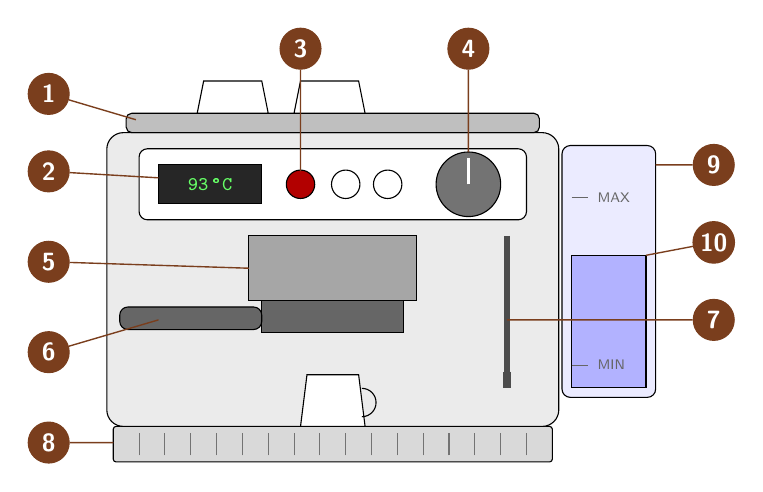
\begin{tikzpicture}[scale=0.82, every node/.style={font=\small},
    callout/.style={circle, draw=brand, fill=brand, text=white, inner sep=1.2pt, minimum size=5.2mm, font=\small\bfseries},
    lead/.style={brand, line width=0.5pt}]
  % drip tray with grille
  \draw[fill=black!15, rounded corners=1pt] (0.1,0) rectangle (6.9,0.55);
  \foreach \x in {0.5,0.9,...,6.5} \draw[black!55, line width=0.4pt] (\x,0.1) -- (\x,0.45);
  % body
  \draw[fill=black!8, rounded corners=6pt] (0,0.55) rectangle (7,5.1);
  % cup warmer
  \draw[fill=black!25, rounded corners=2pt] (0.3,5.1) rectangle (6.7,5.4);
  \draw[fill=white] (1.4,5.4) -- (1.5,5.9) -- (2.4,5.9) -- (2.5,5.4) -- cycle;
  \draw[fill=white] (2.9,5.4) -- (3.0,5.9) -- (3.9,5.9) -- (4.0,5.4) -- cycle;
  % control panel with display, buttons and dial
  \draw[fill=white, rounded corners=3pt] (0.5,3.75) rectangle (6.5,4.85);
  \draw[fill=black!85] (0.8,4.0) rectangle (2.4,4.6);
  \node[text=green!60!white, font=\scriptsize\ttfamily] at (1.6,4.3) {93\,\textdegree C};
  \draw[fill=red!70!black] (3.0,4.3) circle (0.22);
  \draw[fill=white] (3.7,4.3) circle (0.22);
  \draw[fill=white] (4.35,4.3) circle (0.22);
  \draw[fill=black!55] (5.6,4.3) circle (0.5);
  \draw[white, line width=1.2pt] (5.6,4.3) -- (5.6,4.7);
  % group head and portafilter
  \draw[fill=black!35] (2.2,2.5) rectangle (4.8,3.5);
  \draw[fill=black!60] (2.4,2.0) rectangle (4.6,2.5);
  \draw[fill=black!60, rounded corners=3pt] (0.2,2.05) rectangle (2.4,2.4);
  % cup under group head
  \draw[fill=white] (3.0,0.55) -- (3.1,1.35) -- (3.9,1.35) -- (4.0,0.55) -- cycle;
  \draw (3.95,0.7) arc (-90:90:0.22);
  % steam wand
  \draw[line width=2pt, black!70] (6.2,3.5) -- (6.2,1.4);
  \draw[line width=3pt, black!70] (6.2,1.4) -- (6.2,1.15);
  % water tank on the right with level window
  \draw[fill=blue!8, rounded corners=3pt] (7.05,1.0) rectangle (8.5,4.9);
  \draw[fill=blue!30] (7.2,1.15) rectangle (8.35,3.2);
  \draw[black!60, line width=0.4pt] (7.2,4.1) -- (7.45,4.1) node[right, font=\tiny] {MAX};
  \draw[black!60, line width=0.4pt] (7.2,1.5) -- (7.45,1.5) node[right, font=\tiny] {MIN};
  % callouts (number circles with leader lines)
  \node[callout] (c1) at (-0.9,5.7) {1};   \draw[lead] (c1) -- (0.45,5.3);
  \node[callout] (c2) at (-0.9,4.5) {2};   \draw[lead] (c2) -- (0.8,4.4);
  \node[callout] (c3) at (3.0,6.4) {3};    \draw[lead] (c3) -- (3.0,4.5);
  \node[callout] (c4) at (5.6,6.4) {4};    \draw[lead] (c4) -- (5.6,4.8);
  \node[callout] (c5) at (-0.9,3.1) {5};   \draw[lead] (c5) -- (2.2,3.0);
  \node[callout] (c6) at (-0.9,1.7) {6};   \draw[lead] (c6) -- (0.8,2.2);
  \node[callout] (c7) at (9.4,2.2) {7};    \draw[lead] (c7) -- (6.2,2.2);
  \node[callout] (c8) at (-0.9,0.3) {8};   \draw[lead] (c8) -- (0.1,0.3);
  \node[callout] (c9) at (9.4,4.6) {9};    \draw[lead] (c9) -- (8.5,4.6);
  \node[callout] (c10) at (9.4,3.4) {10};  \draw[lead] (c10) -- (8.35,3.2);
\end{tikzpicture}
\end{center}

\begin{tabularx}{\linewidth}{@{}r X r X@{}}
  \toprule
  \textbf{No.} & \textbf{Part} & \textbf{No.} & \textbf{Part} \\
  \midrule
  1 & Cup warming tray & 6 & Portafilter with handle \\
  2 & Display (temperature, program) & 7 & Steam wand with insulated grip \\
  3 & Power button & 8 & Drip tray with removable grille \\
  4 & Program dial (select and confirm) & 9 & Removable water tank (\qty{1.2}{L}) \\
  5 & Group head & 10 & Water level window (MIN and MAX marks) \\
  \bottomrule
\end{tabularx}

\section{Daily use}
\begin{enumerate}[leftmargin=1.6em, itemsep=0.1em]
  \item Fill the water tank (9) with fresh cold water up to the MAX mark and push it firmly back into place.
  \item Press the power button (3). The machine heats up in about \qty{40}{s}; the display (2) shows the
        brewing temperature of \qty{93}{\celsius} when it is ready.
  \item Fill the portafilter (6) with \qty{18}{g} of ground coffee, press it down evenly and lock it into the
        group head (5).
  \item Place a cup on the drip tray (8) and press the program dial (4). A double espresso of about
        \qty{36}{g} in the cup takes roughly \qty{28}{s}.
\end{enumerate}

\begin{cautionbox}
Never remove the portafilter while water is flowing. The steam wand (7) stays hot for several minutes after
use; wipe it with a damp cloth and purge it for two seconds after every use.
\end{cautionbox}

\section{Descaling}
Limescale reduces the heating performance, the water flow and the taste of your coffee. Descale the machine
regularly. The display shows \texttt{dESC} after 200 brewing cycles. The interval depends on your local water
hardness:

\begin{center}
\begin{tabular}{@{}l l l@{}}
  \toprule
  \textbf{Water hardness} & \textbf{Range} & \textbf{Descale every} \\
  \midrule
  Soft & 0 to \qty{7}{\degree dH} & 6 months \\
  Medium & 8 to \qty{14}{\degree dH} & 3 months \\
  Hard & above \qty{14}{\degree dH} & 6 weeks \\
  \bottomrule
\end{tabular}
\end{center}

\begin{warnbox}
The descaling solution irritates eyes and skin. Wear protective gloves and avoid contact. If the solution
gets into your eyes, rinse them with plenty of water for at least 15 minutes and consult a doctor. Never
drink the solution and never leave the machine unattended while descaling.
\end{warnbox}

\begin{cautionbox}
Use only the Morvale descaler (art. no.\ MV-DS30) or a descaler based on citric acid. Never use vinegar,
lemon juice or descalers containing sulfamic acid or hydrochloric acid; they damage the boiler and void the
warranty.
\end{cautionbox}

\subsection{Procedure}
You need one sachet of Morvale descaler (\qty{30}{g}) and a container that holds at least \qty{1}{L}.
\begin{enumerate}[leftmargin=4.4em, itemsep=0.25em, label=\textbf{Step \arabic*.}, labelsep=0.6em]
  \item Switch the machine off. Remove the water tank (9) and, if fitted, the water filter. Empty the drip tray (8).
  \item Dissolve one sachet of descaler (\qty{30}{g}) in \qty{0.8}{L} of lukewarm water. Pour the solution
        into the water tank and put the tank back.
  \item Remove the portafilter (6). Place the container under the group head (5) and the steam wand (7) so that
        both outlets point into it.
  \item Switch the machine on. Turn the program dial (4) to \texttt{dESC} and hold it pressed for
        \qty{3}{s}. The programme now runs for about \qty{25}{min}, with pauses, and releases the solution in
        stages through the group head and the steam wand.
  \item When the machine beeps three times and the display shows \texttt{rinS}, the descaling is finished.
        Empty the container.
  \item Rinse the tank thoroughly, fill it with \qty{1.2}{L} of fresh cold water and press the program dial
        to start the rinse cycle. Repeat the rinse once with a second full tank, so that \qty{2.4}{L} of fresh
        water have passed through the machine in total.
  \item Refit the water filter, empty the drip tray and reset the counter: hold the dial pressed for
        \qty{5}{s} while the display shows \texttt{rSET}. Brew one espresso and discard it before you drink coffee again.
\end{enumerate}

\Needspace{16\baselineskip}
\section{Troubleshooting}
If your machine does not work as expected, check the table before you contact customer service.

\begin{center}
\small
\captionof{table}{Troubleshooting guide}
\begin{tabularx}{\linewidth}{@{}>{\raggedright\arraybackslash}p{3.6cm} >{\raggedright\arraybackslash}X >{\raggedright\arraybackslash}X@{}}
  \toprule
  \textbf{Problem} & \textbf{Possible cause} & \textbf{Remedy} \\
  \midrule
  Machine does not switch on & Plug not connected, no mains power & Check the plug and the outlet. If the machine still does not start, contact customer service. \\
  \addlinespace[2pt]
  No water from the group head & Tank empty or not seated; boiler scaled & Fill the tank, push it in firmly. If the problem remains, descale the machine. \\
  \addlinespace[2pt]
  Espresso runs through in less than \qty{15}{s} & Grind too coarse or too little coffee & Use a finer grind and \qty{18}{g} of coffee. \\
  \addlinespace[2pt]
  Espresso drips slowly, takes more than \qty{40}{s} & Grind too fine or tamped too hard & Use a coarser grind and press more lightly. \\
  \addlinespace[2pt]
  Weak steam, milk does not foam & Steam nozzle blocked & Let the wand cool, then clean the nozzle with a fine needle and purge for two seconds. \\
  \addlinespace[2pt]
  Display shows \texttt{dESC} & 200 brewing cycles reached & Descale the machine (section 4). \\
  \addlinespace[2pt]
  Display shows \texttt{E04} & Boiler overheated & Switch off and wait \qty{30}{min}. If the error returns, contact customer service. \\
  \addlinespace[2pt]
  Water under the machine & Drip tray full or tank not seated & Empty the drip tray and reseat the tank. If water keeps leaking, unplug the machine. \\
  \bottomrule
\end{tabularx}
\end{center}

\section{Technical specifications}
\begin{center}
\captionof{table}{Technical specifications of the Morvale ES-300}
\begin{tabular}{@{}l l@{\hspace{3em}}l l@{}}
  \toprule
  \textbf{Feature} & \textbf{Value} & \textbf{Feature} & \textbf{Value} \\
  \midrule
  Rated voltage & 220 to \qty{240}{V}, 50/60 Hz & Brewing temperature & \qty{93}{\celsius} (adjustable 88 to \qty{96}{\celsius}) \\
  Rated power & \qty{1450}{W} & Heat-up time & about \qty{40}{s} \\
  Pump pressure & \qty{15}{bar} & Max.\ cup height & \qty{11}{cm} \\
  Water tank & \qty{1.2}{L} & Dimensions (W $\times$ D $\times$ H) & 28 $\times$ 31 $\times$ 34 cm \\
  Cable length & \qty{1.0}{m} & Weight (empty) & \qty{5.8}{kg} \\
  Protection class & I & Noise level & \qty{56}{dB(A)} \\
  \bottomrule
\end{tabular}
\end{center}

\subsection*{Disposal and warranty}
Do not dispose of the machine with household waste; take it to a collection point for electrical equipment. The
legal warranty period is 24 months from the date of purchase. Keep the receipt.

\end{document}
